Рассмотрим первый проимер.

Базза начинает игру со следующих ходов:
\begin{itemize}
\item присваивает ячейке $(0, 0)$ число $20$;
\item присваивает ячейке $(0, 2)$ число $15$; присваивает ячейке $(1, 1)$ число $12$.
\end{itemize}


\includegraphics{1.png}

Получившаяся таблица показана на рисунке выше. Базза далее задает вопрос, чему равен НОД внутри следующих прямоугольников:
\begin{itemize}
\item с противоположными углами $(0, 0)$ и $(0, 2)$ (в этом прямоугольнике три числа~--- $20$, $0$ и $15$, и их НОД равен $5$);
\item с противоположными углами $(0, 0)$ и $(1, 1)$ (в этом прямоугольнике четыре числа~--- $20$, $0$, $0$ и $12$, и их НОД равен $4$).
\end{itemize}

Далее Базза делает следующие ходы:
\begin{itemize}
\item присваивает ячейке $(0, 1)$ число $6$;
\item присваивает ячейке $(1, 1)$ число $14$.
\end{itemize}

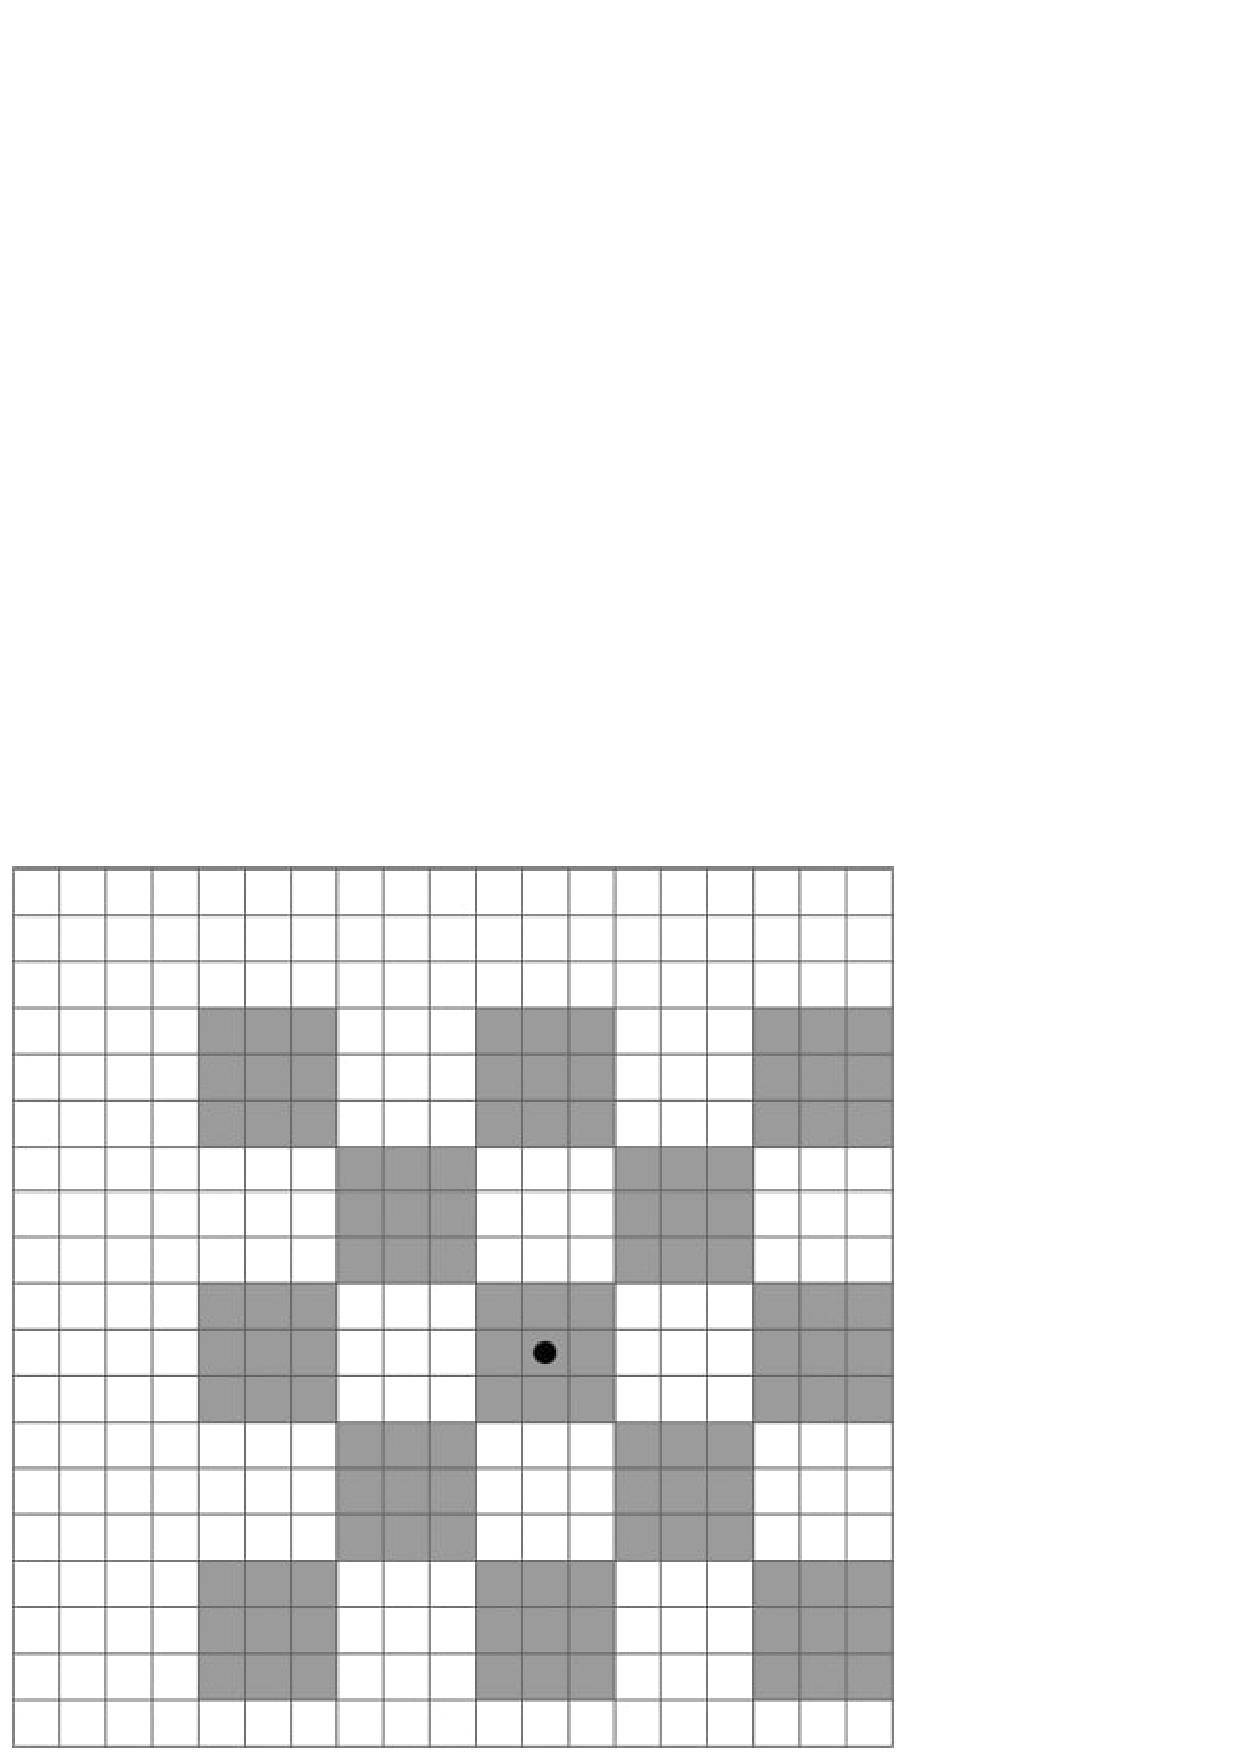
\includegraphics{2.png}

Новая таблица показана на рисунке выше. Базза далее задает вопрос, чему равен НОД внутри следующих прямоугольников:
\begin{itemize}
\item с противоположными углами $(0, 0)$ и $(0, 2)$ (теперь в этом прямоугольнике три числа~--- $20$, $6$ и $15$, и их НОД равен $1$);
\item с противоположными углами $(0, 0)$ и $(1, 1)$ (теперь в этом прямоугольнике четыре числа~--- $20$, $6$, $0$ и $14$, и их НОД равен $2$).
\end{itemize}